This section will describe how we used the project backlog, as well as how we handled each sprint. \\

The project backlog can be seen in \autoref{fig:projectBacklog}. \\

Our project backlog consists of: 
\begin{description}
  \item[Column 1:] An ID for the assignment
  \item[Column 2:] A name 
  \item[Column 3:] A priority from 1-10, 1 being the highest
  \item[Column 4:] An estimate of the time taken
  \item[Column 5:] A ``how to demo'' description
  \item[Column 6:] A possible note
  \item[Column 7:] A status
\end{description}
Note that time taken is not actual hours but a relative value. This means that an assignment with the value 4 should take twice as long as an assignment with the value 2, but not necessarily take 4 and 2 hours respectively.

The project backlog is divided into colors. The colors represent which sprint the assignment was added, starting with before sprint 1, during sprint 1, before sprint 2, during sprint 2 etc. The status attribute has four values: Not started, Completed, Waiting for external source, and In progress.

The project backlog was a new tool for us this semester, therefore we had some issues in the start of the project, which we gradually managed to solve. The main issues were the estimation of time and vaguely defined assignments. 

Our first version of the backlog was short and unspecific, with large assignments, which made it hard to estimate the implementation time. We felt like no progress was made, as we did not finish most of the planned assignments during the sprint. To counteract this, we started splitting our assignments into smaller more concrete assignments. This made it easier for us to estimate the time, and we started to finish more assignments during a sprint giving a feeling of progress. 

An example of this is the web interface: It was defined as two assigments called ``Web Interface: GUI Design'' and ``Web Interface: CRUD Management''. These two assignments cover the whole web interface of our project. Even though we gave them a big time estimate of 20 and 10 respectivly, this was nowhere near enough time to finish it. These two assignments kept being in the ``In progress'' state for quite some time. After that, we decided to split the two assignments into more concrete assigments. This resulted in 20 simpler assignments like ``Profile: add'' or ``Tags: delete''. 

Our sprints reflects this progress of experience as well

\begin{description}
\item [Sprint 1, from 19/03/2012 to 23/03/2012]
	During this sprint we focu-sed on the database and the sw6ml\footnote{XML language for Savannah \autoref{sw6ml}} schema. We wanted to start out light because we had no experience with how much we were capable of doing, during one sprint. We decided that it was better to start with fewer assignment on the sprint backlog, and then add assignments if necessary, rather than struggling to finish everything in the sprint. We found that we could easily finish what we had added to the sprint backlog, but this was mainly because we had done a lot of work prior to the sprint, so much of the work was already done.
\item[Sprint 2, from 26/03/2012 to 04/04/2012]
	During this sprint we star-ted working on the design of the web interface. We also had to update the sw6ml schema and the database to new requirements. Server data I/O and transmission packages was also worked on in this sprint. In the end of the sprint we had a mock up of our web interface for our contact to see, therefore we contacted her to schedule a meeting and receive feedback before the beginning of the next sprint. The meeting went well and we got some feedback that was added on to our requirements list. 
\item[Sprint 3, from 10/04/2012 to 19/04/2012]
	In this sprint we worked on the CRUD capabilities for the server to communicate with the database. We also had to update the database design and sw6ml schema again to meet new requirements. The server controller,the main class of the server, was also planed as well as to create the Savannah data API. For the web interface we had two assignments: Update the design to meet the new requirements, and implement the web interface on the Tomcat\footnote{A web server with Servlet support} server. We realized that the complexity of the web interface was higher than estimated, and we did not finish anything web interface related.
\item [Sprint 4, from 23/04/2012 to 02/05/2012]
	In this sprint we added a lot of assignments to the project backlog. This sprint's backlog was unlike the previous, in that it had almost trice as many assignments. This was because of the assignment reassessment: All the assignments were smaller and more manageable. Even though there were almost trice as many assignments, we also finished more assignments during the sprint.
\item[Remaining sprints, 5 to 7]
	Sprint 4 became our last organized sprint. The reason for this was that no more assignments were added to the project backlog so we had a clear overview of what needed to be done. We started to focus on finishing current work, instead of adding new features. This resulted in us not utilizing the sprint backlog. We started working together with the other groups to make a release, and to plan the usability test, which was carried out in sprint 6. In this period we also started working on an assignment, which had been on our project backlog through the entire project: Writing the report.  
\end{description}

\begin{figure}
 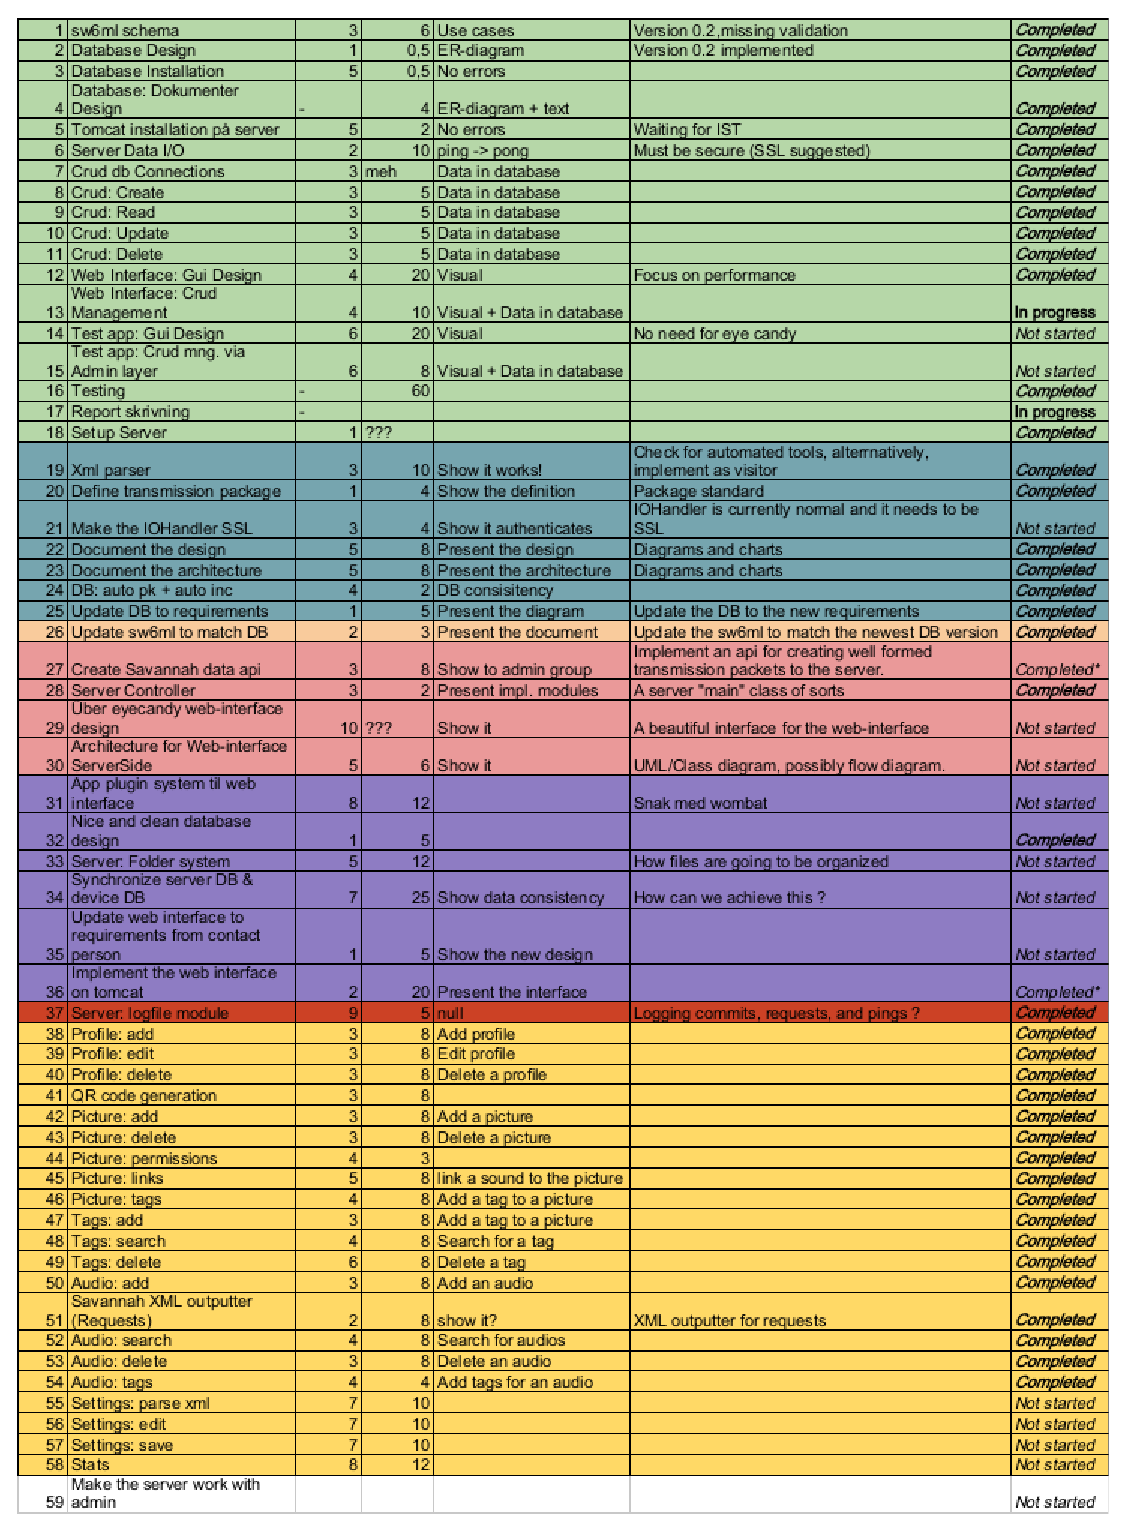
\includegraphics[scale=0.72]{images/projectBacklog}
 \caption{Project backlog.}
 \label{fig:projectBacklog}
\end{figure}

Working in sprints has yielded positive results for the multi project, as all groups have had great knowledge of what the other groups were doing, and when they could expect certain features to be finished. 